\documentclass[]{article}
\usepackage{lmodern}
\usepackage{amssymb,amsmath}
\usepackage{ifxetex,ifluatex}
\usepackage{fixltx2e} % provides \textsubscript
\ifnum 0\ifxetex 1\fi\ifluatex 1\fi=0 % if pdftex
  \usepackage[T1]{fontenc}
  \usepackage[utf8]{inputenc}
\else % if luatex or xelatex
  \ifxetex
    \usepackage{mathspec}
  \else
    \usepackage{fontspec}
  \fi
  \defaultfontfeatures{Ligatures=TeX,Scale=MatchLowercase}
\fi
% use upquote if available, for straight quotes in verbatim environments
\IfFileExists{upquote.sty}{\usepackage{upquote}}{}
% use microtype if available
\IfFileExists{microtype.sty}{%
\usepackage{microtype}
\UseMicrotypeSet[protrusion]{basicmath} % disable protrusion for tt fonts
}{}
\usepackage[margin=1in]{geometry}
\usepackage{hyperref}
\hypersetup{unicode=true,
            pdftitle={Predicting Real Estate Sales Using Machine Learning and Spatial Dependence},
            pdfborder={0 0 0},
            breaklinks=true}
\urlstyle{same}  % don't use monospace font for urls
\usepackage{longtable,booktabs}
\usepackage{graphicx,grffile}
\makeatletter
\def\maxwidth{\ifdim\Gin@nat@width>\linewidth\linewidth\else\Gin@nat@width\fi}
\def\maxheight{\ifdim\Gin@nat@height>\textheight\textheight\else\Gin@nat@height\fi}
\makeatother
% Scale images if necessary, so that they will not overflow the page
% margins by default, and it is still possible to overwrite the defaults
% using explicit options in \includegraphics[width, height, ...]{}
\setkeys{Gin}{width=\maxwidth,height=\maxheight,keepaspectratio}
\IfFileExists{parskip.sty}{%
\usepackage{parskip}
}{% else
\setlength{\parindent}{0pt}
\setlength{\parskip}{6pt plus 2pt minus 1pt}
}
\setlength{\emergencystretch}{3em}  % prevent overfull lines
\providecommand{\tightlist}{%
  \setlength{\itemsep}{0pt}\setlength{\parskip}{0pt}}
\setcounter{secnumdepth}{0}
% Redefines (sub)paragraphs to behave more like sections
\ifx\paragraph\undefined\else
\let\oldparagraph\paragraph
\renewcommand{\paragraph}[1]{\oldparagraph{#1}\mbox{}}
\fi
\ifx\subparagraph\undefined\else
\let\oldsubparagraph\subparagraph
\renewcommand{\subparagraph}[1]{\oldsubparagraph{#1}\mbox{}}
\fi

%%% Use protect on footnotes to avoid problems with footnotes in titles
\let\rmarkdownfootnote\footnote%
\def\footnote{\protect\rmarkdownfootnote}

%%% Change title format to be more compact
\usepackage{titling}

% Create subtitle command for use in maketitle
\newcommand{\subtitle}[1]{
  \posttitle{
    \begin{center}\large#1\end{center}
    }
}

\setlength{\droptitle}{-2em}
  \title{Predicting Real Estate Sales Using Machine Learning and Spatial
Dependence}
  \pretitle{\vspace{\droptitle}\centering\huge}
  \posttitle{\par}
\subtitle{Boosting Random Forest Predictive Accuracy Using Spatial Lags}
  \author{}
  \preauthor{}\postauthor{}
  \date{}
  \predate{}\postdate{}

\setlength{\parindent}{0em}
\setlength{\parskip}{1em}

\begin{document}
\maketitle

{
\setcounter{tocdepth}{2}
\tableofcontents
}
\section{Introduction}\label{introduction}

\subsection{What is Economic
Exclusion?}\label{what-is-economic-exclusion}

Income inequality may be a defining challenge of our time. Researchers
at the Urban Institute (Solomon Greene and Lei 2016) recently identified
the socio-economic phenomenon of ``Economic Exclusion'' as one
compelling explanation for the recent rise in inequality in the US. As
discussed by Zuk (2015), ``Neighborhoods change slowly, but over time
are becoming more segregated by income, due in part to macro-level
increases in income inequality''. Vulnerable
populations--disproportionately communities of color, immigrants,
refugees, and women--who are displaced by localized economic prosperity
enter into a gradual cycle of diminished access to good jobs, good
schools, health care facilities, public spaces, etc. Such systematic
denial causes enduring and self-reinforcing poverty over the course
years and even generations, gradually entrenching income inequality and
general unrest.

One way to practically combat economic exclusion is to focus on
preventing displacement, however, detecting gentrification at an early
enough stage can be a daunting task. When an area experiences economic
growth, increased housing demands and subsequent affordability pressures
can lead to evictions of low-income families and small businesses.
Government agencies and nonprofits tend to intervene once displacement
is already underway, and after-the-fact interventions can be costly and
ineffective. There are a host of preemptive actions that can be deployed
to stem divestment and ensure that existing residents benefit from new
investments. Not unlike medical treatment, early detection is key to
success. Consequently, in 2016, the Urban Institute put forth a call for
research into the creation of ``neighborhood-level early warning and
response systems that can help city leaders and community advocates get
ahead of neighborhood changes'' (2016).

(M. Chapple Karen; Zuk 2016) To be included in the ``motivation''
section of my thesis. Not about predictive modeling, but is a very
recent overview of the application of predictive gentrification models

\subsection{How Can Machine Learning
Help?}\label{how-can-machine-learning-help}

Predictive modeling using spatial dependence has been employed
extensively in recent years, notably in Crime Prediction (Almanie 2015).
However, a key deficiency of many spatial models are their use of
arbitrarily defined geographic regions, such as zip codes, political
districts, police precincts, state lines, neighborhoods, etc. which
diminish and obscure potentially valuable insights. Worse yet, many
predictive models ignore spatial dependence, violating one of the basic
tenets of geography: the direct relationship between distance and
likeness (Miller 2007).

\subsection{Our Contribution}\label{our-contribution}

This paper explores novel techniques to predict gentrification in the
pursuit of combating displacement and economic exclusion. Modern
techniques of data mining, machine learning and predictive modeling are
applied to data sets describing property values and sale prices in New
York City. We demonstrate that the incorporation of spatial lags, i.e.,
variables created from physically proximate observations, can improve
the predictive accuracy of machine learning models above and beyond both
non-spatial models as well as models which incorporate data aggregated
at arbitrary geographic regions such as zip codes.

\section{Literature Review}\label{literature-review}

The literature review for this paper reviews the concept of Economic
Displacement as it has been addressed in academia, primarily in relation
to the study of gentrification. We also examine ``mass appraisal
techniques'', which are automated analytical techniques used for valuing
large numbers of real estate properties. Finally, we will briefly
examine machine learning as it relates to the problem of predicting
gentrification and/or Economic Displacement.

\subsection{How Has Economic Displacement Been Addressed in the
Past?}\label{how-has-economic-displacement-been-addressed-in-the-past}

Economic Displacement has been intertwined with the study of
gentrification since shortly after the latter became academically
relevant in the 1960's. The term ``gentrification'' was first used by
Ruth Glass in 1964 to described the ``gentry'' in low income
neighborhoods in London. Gentrification was originally understood as a
``tool of revitalization for declining neighborhoods'' (Zuk 2015),
however, in 1979 Phillip Clay made the distinction between two types of
revitalization: ``incumbent upgrading'' and ``gentrification'', noting
that Economic Displacement was the negative consequence of the latter
(Clay 1979). Today, the term has evolved to describe ``a spatial
organization and re-organization of human dwelling and activity'' (Zuk
2015). Specific to cities, gentrification is thought of as ``the
transformation of a working-class or vacant area of the central city
into middle-class residential or commercial use'' (Lees 2008).

Studies of gentrification and displacement generally take two approaches
in the literature: supply-side and demand-side, or ``the flows of
capital versus flows of people to neighborhoods'', respectively (Zuk
2015). Supply side arguments for gentrification tend to focus on
``private capital investment, public policies, and public investments''
(Zuk 2015). (Smith 1979) argued that the return of capital from the
suburbs to the city drives gentrification. He describes a ``political
economy of capital flows into urban areas'' (Zuk 2015) as largely
responsible for both the positive and negative consequences of
gentrification. According to (Dreier 2004), public policies that have
been linked to increased Economic Displacement have been, among others,
automobile-oriented transportation infrastructure spending and mortgage
interest tax deductions for home owners.

More recently, income inequality has been explored as a major
contributor to Economic Displacement, specifically, ``higher
compensation in the top quintile and the lack of jobs for the bottom
quintile'' (Reardon 2011); (Watson 2009). The concentration of wealth
allows ``certain households to sort themselves according to their
preferences -- and control local political processes that continue
exclusion'' (Reardon 2011). This results in a self-reinforcing feedback
loop where wealthier households influence public policy toward their
self interest. Gentrification prediction tools could be used to help
break such feedback loops through early identification and intervention.
Reardon (2011) also argues that ``were income inequality to stop rising,
the number of segregated neighborhoods would decline.''

Many studies conclude that gentrification in most forms leads to
exclusionary economic displacement, however, Zuk (2015) characterizes
the results of many recent studies as ``mixed, due in part to
methodological shortcomings''. In this paper, we attempt to further the
understanding of gentrification prediction by demonstrating a technique
to better predict real estate sales in New York City.

\subsection{A Review of Mass Appraisal
Techniques}\label{a-review-of-mass-appraisal-techniques}

Much of the research on predicting real estate prices has been in
service of creating mass appraisal models. Mass appraisal models are
most commonly used by local governments for the purpose of collecting
taxes from property owners. Mass appraisal models share many
characteristics with predictive machine learning models, in that they
are data-driven, standardized methods that employ statistical testing
(Eckert 1990). A variation on mass appraisal models are the ``automated
valuation models'' (AVM), which use ``often the same methodological
framework of mass appraisal\ldots{} a statistical model and a large
amount of property data to estimate the market value of an individual
property or portfolio of properties'' (d'Amato 2017).

Scientific mass appraisal models date back to 1936 with the reappraisal
of St.~Paul, Minnesota (Silverherz 1936). Since that time, and
accelerated with the advent of computers, much statistical research has
been done relating property values and rent prices to various
characteristics of those properties, including characteristics of their
surrounding area. Multiple regression analysis (MRA) has been the most
common set of statistical tools used in mass appraisal, including
Maximum Likelihood, Weighted Least Squares, and the most popular,
Ordinary Least Squares (OLS) (d'Amato 2017). The primary drawbacks of
MRA techniques are ``excessive multicollinearity among attributes'' and
``spatial autocorrelation among residuals'' (d'Amato 2017). Another
group of models that seek to correct for spatial dependence are known as
Spatial Auto Regressive (SAR) models, chief among them the Spatial Lag
Model, which aggregates weighted summaries of nearby properties in order
to create independent regression variables (d'Amato 2017).

Hedonic regression models generally seek to break down the price of a
good based on the intrinsic and extrinsic components. Koschinsky (2012)
is a recent and thorough discussion of parametric hedonic regression
techniques. Some of the variables included in Koschinsky's models are
derived from nearby properties, similar to the technique used in this
paper, and these variables were found to be predictive. The real estate
hedonic model as defined by Koschinsky describes the price of a property
as:

\[
\begin{aligned}
 P_i = P(S_i, N_i, L_i)
\end{aligned}
\]

Where \(P_i\) represents the price of house \(i\), which is a composite
good comprised of a vector of structural characteristics \(S\), a vector
of social and neighborhood characteristics \(N\), and a vector of
locational characteristics \(L\). Specifically, the model calculates
spatial lags on properties of interest using neighboring properties
within 1,000 feet of a sale. The derived variables include
characteristics like average age, quantity of poor condition homes,
percent of homes with electric heating, construction grade, etc. within
1,000 feet of the property in question. Koschinsky found that in all
cases, ``the relation between a home's price and the average price of
its neighboring homes is characterized by positive spatial
autocorrelation'' meaning that homes near each other were typically
similar to each other and priced accordingly. Koschinsky concluded that
locational characteristics should be valued at least as much ``if not
more'' than important structural characteristics.

As recently as 2015, much research has dealt with mitigating the
drawbacks of MRA, including the use of multi-level hierarchical models.
Fotheringham (2015) explored the combination of Geographically Weighted
Regression (GWR) with time-series forecasting to predict home prices
over time. GWR is a variation on OLS that allows for ``adaptive
bandwidths'' of local data to be included, i.e., for each estimate, the
number of data points included varies and can be optimized using
cross-validation.

Automated valuation modeling got a legal update in the aftermath of the
2008 financial crisis by way of the The Dodd Frank Act. In particular,
the Title XIV, subtitle F distinguishes the ``appraisal'' process from
automated valuation modelling, and reorganized both (d'Amato 2017). The
Act asserts that appraisal, or valuation conducted by a human being,
cannot be replaced by AVM. At current, AVM is ``increasingly adaptable
in describing real estate market behavior'' but has yet to supersede the
importance and necessity of local information and human evaluation.

\subsection{Has Machine Learning Been Applied to this Problem
Before?}\label{has-machine-learning-been-applied-to-this-problem-before}

Both Mass Appraisal techniques and Automated Valuation Modeling seek to
predict real estate prices using data and statistical methods, however,
traditional techniques typically fall short of reality. This is because
property valuation is inherently a ``chaotic'' process that does not
lend itself to binary or linear analysis (Zuk 2015). The value of any
given property is a complex combination of perceived value and
speculation. The value of any building or plot of land belongs to a rich
network where decisions about and perceptions of neighboring properties
influence the final market value. Guan et al. (2014) compared
traditional MRA techniques to alternative ``data mining techniques''
resulting in ``mixed results''. However, as Helbich (2013) states,
hedonic pricing models ``can be improved in two ways: (a) Through novel
estimation techniques, and (b) by ancillary structural, locational, and
neighborhood variables on the basis of Geographic Information System
(GIS)''. Recent research generally falls into these two buckets: better
analysis algorithms and/or better data.

In the ``better data'' category, researchers have been striving to
introduce new independent variables to increase the accuracy of
predictive models. Dietzell (2014) successfully used internet search
query data provided by Google Trends to serve as a sentiment indicator
and improve commercial real estate forecasting models. Pivo and Fisher
(2011) examined the effects of walkability on property values and
investment returns. Pivo found that on a 100-point scale, a 10-point
increase in walkability increased property investment values by up to
9\%.

Research into better prediction algorithms do not necessarily happen at
the exclusion of ``better data''. For example, Fu (2014) created a
prediction algorithm, called ``ClusRanking'', for real estate in
Beijing, China. ClusRanking first estimates neighborhood characteristics
using taxi cab traffic vector data, specifically as they relate to
accessibility to ``business areas''. Then, the algorithm performs a
rank-ordered prediction of investment returns segmented into five
categories. Similar to Koschinsky (2012), though less formally stated,
Fu (2014) thought of a property's value as a composite of individual,
peer and zone characteristics. In the predictive model, Fu includes
characteristics of the neighborhood (individual), the values of its
nearby properties (peer), and the prosperity of the affiliated latent
business area (zone) based on taxi cab data (Fu 2014).

Several other recent studies compare various ``advanced'' statistical
techniques and algorithms either to other advanced techniques or to
traditional ones. Most studies conclude that the advanced,
non-parametric techniques outperform traditional parametric techniques,
while several conclude that the Random Forest algorithm is particularly
well-suited to predicting real estate values.

Kontrimasa (2011) compares the accuracy of linear regression against the
SVM technique and found the latter to outperform. Schernthanner H.
(2016) compared traditional linear regression techniques to several
techniques such as krigging (stochastic interpolation) and Random
Forest. They concluded that the more advanced techniques, particularly
random forest, are sound and more accurate when compared to traditional
statistical methods. Antipov and Pokryshevskaya (2012) comes to a
similar conclusion about the superiority of Random Forest to real estate
valuation after comparing 10 algorithms: multiple regression, CHAID,
Exhaustive CHAID, CART, 2 types of k-Nearest Neighbors, Multilayer
Perceptron neural network (MLP), Radial Basis Function neural network
(RBF)), Boosted Trees and finally Random Forest.

Guan et al. (2014) compared three different approaches to defining
spatial neighbors: a simple radius technique, a k-nearest neighbors
technique using only distance and a k-nearest neighbors technique using
all attributes. Interestingly, the location-only KNN models performed
best, although by a slight margin. Park (2015) developed several housing
price prediction models based on machine learning algorithms including
C4.5, RIPPER, Naive Bayesian, and AdaBoost. By comparing the models'
classification accuracy performance, the experiments demonstrate that
the RIPPER algorithm, based on accuracy, consistently outperformed the
other models in the performance of housing price prediction. Rafiei
(2016) employed a restricted boltzmann machine (neural network with back
propagation) to predict the sale price of residential condos in Tehran,
Iran. Rather than focusing on predictive performance, their paper
focuses on computational efficiency. A non-mating genetic algorithm is
used for dimensionality reduction. The paper concludes that two primary
strategies help in this regard: weighting property sales by temporal
proximity (sales which happened closer in time are more important), and
also using a learner to accelerate the recognition of important
features. The paper compares this technique to several other common
neural network approaches and finds that while not necessarily the only
way to get the best answer, it is the fastest way to get to the best
answer.

Finally, it should be noted that many studies, whether exploring
advanced techniques, new data, or both, rely on aggregation of data by
some arbitrary boundary. For example, Turner and Snow (2001) predicted
gentrification in the Washington, D.C. metro area by ranking census
tracts in terms of development. K. Chapple (2009) created a
gentrification ``early warning system'' by identifying low income census
tracts in central city locations. Barry Bluestone \& Chase Billingham
(2010) analyzed 42 census block groups near rail stations in 12 metro
areas across the United States, studying changes between 1990 and 2000
for neighborhood socioeconomic and housing characteristics. All of these
studies, and many more, relied on aggregation of data at the
census-tract or census-block level. In contrast, this paper compares
boundary-aggregation techniques (specifically, aggregating by zip codes)
to spatial-lag techniques and finds the spatial lag techniques to
generally outperform.

\section{Methodology}\label{methodology}

Our goal is to compare the use of spatial lags as features in a machine
learning predictive model against traditional feature engineering
techniques. We will create three modeling data sets:

\begin{itemize}
\tightlist
\item
  Base
\item
  Zip Code
\item
  Spatial Lag
\end{itemize}

We will then create 2 predictive models for each modeling data set,
using a different outcome variable for each:

\begin{enumerate}
\def\labelenumi{\arabic{enumi})}
\tightlist
\item
  Probability of Sale. The probability that a given property in New York
  City will sell in a given year
\item
  Amount of Sale. Given that a property sells, how much is the sale
  value?
\end{enumerate}

There will be six predictive models built in total, as follows:

\begin{longtable}[]{@{}rllllll@{}}
\toprule
\# & Model & Model Type & Data & Outcome Variable & Outcome Var Type &
Evaluation Metric\tabularnewline
\midrule
\endhead
1 & Probability of Sale & Classification & Base & Building Sold & Binary
& AUC\tabularnewline
2 & Probability of Sale & Classification & Zip Code & Building Sold &
Binary & AUC\tabularnewline
3 & Probability of Sale & Classification & Spatial Lags & Building Sold
& Binary & AUC\tabularnewline
4 & Sale Price & Regression & Base & Sale Price per SF & Continuous &
RMSE\tabularnewline
5 & Sale Price & Regression & Zip Code & Sale Price per SF & Continuous
& RMSE\tabularnewline
6 & Sale Price & Regression & Spatial Lag & Sale Price per SF &
Continuous & RMSE\tabularnewline
\bottomrule
\end{longtable}

To accomplish this, we combine three open-source data repositories
provided by New York City via \url{nyc.gov} and
\url{data.cityofnewyork.us}. Our base modeling data set includes all
building records and associated sales information from 2003-2017.

Following the creation of the base modeling data, we create two
additional data sets through feature engineering: a ``Zip Code
features'' data set and a ``Spatial Lag features'' data set. The primary
goal of this study is to compare the predictive power of the spatial
lags vs.~the base and zip code features.

\subsection{Data}\label{data}

The New York City government makes available an annual data set which
describes all tax lots in the five boroughs. The Primary Land Use and
Tax Lot Output data set, known as
\href{https://www1.nyc.gov/site/planning/data-maps/open-data/bytes-archive.page?sorts\%5Byear\%5D=0}{PLUTO},
contains a single record for every tax lot in the city along with a
number of building and tax-related attributes such as Year Built,
Assessed Value, Square Footage, number of stories, and many more. At the
time of this writing, NYC has made this data set available for all years
between 2002-2017, excluding 2008. For convenience, we also exclude the
2002 data set from our analysis because sales information is not
available for that year. Importantly for our analysis, the latitude and
longitude of the tax lots are also made available, allowing us to locate
in space each building and to build geospatial features from the data.

Ultimately, we are interested in sales transactions--both frequency, and
amount. Sales transactions are also made available by the New York City
government, known as
\href{http://www1.nyc.gov/site/finance/taxes/property-annualized-sales-update.page}{NYC
Rolling Sales Data}. At the time of this writing, sales transactions are
available for the years 2003-2017. The sales transactions data contains
additional data fields describing time, place, and amount of sale as
well as additional building characteristics. Crucially, the sales
transaction data does not include geographical coordinates, making it
impossible to perform geospatial analysis without first mapping the
sales data to PLUTO.

Prior to mapping to PLUTO, the sales data must first be transformed to
include the proper mapping key. New York City uses a standard key of
Borough-Block-Lot to identify tax lots in the data. For example, 31 West
27th Street is located in Manhattan, on block 829 and lot 16, therefore,
its Borough-Block-Lot (BBL) is 1\_829\_16 (the 1 represents Manhattan).
The sales data contains BBL's at the building level, however, the sales
transactions data does not appropriately designate condos as their own
BBLs. Mapping the sales data directly to the PLUTO data results in a
mapping error rate of 23.1\%. Therefore, the sales transactions data
must first be mapped to another data source, the NYC Property Address
Directory, or
\href{https://data.cityofnewyork.us/City-Government/Property-Address-Directory/bc8t-ecyu/data}{PAD}),
which contains an exhaustive list of all BBLs in NYC. Once the sales
data is combined with PAD, the data can be mapped to PLUTO with an error
rate of 0.291\%.

After the Sales Transactions data has been mapped to PAD, it can then be
mapped to PLUTO. The sales data is normalized and filtered so that only
BBLs with less than or equal to 1 transactions in a year occur. The
final data set is an exhaustive list of all tax lots in NYC for every
year between 2003-2017, whether that building was sold, for what amount,
and several other additional variables.

Only building categories of significant interest are included in the
data. The following building types are included:

\begin{longtable}[]{@{}ll@{}}
\toprule
Category & Description\tabularnewline
\midrule
\endhead
A & ONE FAMILY DWELLINGS\tabularnewline
B & TWO FAMILY DWELLINGS\tabularnewline
C & WALK UP APARTMENTS\tabularnewline
D & ELEVATOR APARTMENTS\tabularnewline
F & FACTORY AND INDUSTRIAL BUILDINGS\tabularnewline
G & GARAGES AND GASOLINE STATIONS\tabularnewline
L & LOFT BUILDINGS\tabularnewline
O & OFFICES\tabularnewline
\bottomrule
\end{longtable}

The data is further filtered to include only records with equal to or
less than 2 buildings per tax lot. The global filtering of the data set
reduces the base modeling data from 12,012,780 records down to
8,247,499.

\subsection{Feature Engineering}\label{feature-engineering}

\subsubsection{Base modeling data}\label{base-modeling-data}

The base modeling data set is enhanced to include additional features. A
summary table of the additional features are presented below:

\begin{longtable}[]{@{}lllll@{}}
\toprule
Feature & Min & Median & Mean & Max\tabularnewline
\midrule
\endhead
has\_building\_area & 0 & 1.00 & 1.00 & 1.00\tabularnewline
Percent\_Com & 0 & 0.00 & 0.16 & 1.00\tabularnewline
Percent\_Res & 0 & 1.00 & 0.82 & 1.00\tabularnewline
Percent\_Office & 0 & 0.00 & 0.07 & 1.00\tabularnewline
Percent\_Retail & 0 & 0.00 & 0.04 & 1.00\tabularnewline
Percent\_Garage & 0 & 0.00 & 0.01 & 1.00\tabularnewline
Percent\_Storage & 0 & 0.00 & 0.02 & 1.00\tabularnewline
Percent\_Factory & 0 & 0.00 & 0.00 & 1.00\tabularnewline
Percent\_Other & 0 & 0.00 & 0.00 & 1.00\tabularnewline
Last\_Sale\_Price & 0 & 312.68 & 531.02 & 62,055.59\tabularnewline
Last\_Sale\_Price\_Total & 2 & 2,966,835.00 & 12,844,252.00 &
1,932,900,000.00\tabularnewline
Years\_Since\_Last\_Sale & 1 & 4.00 & 5.05 & 14.00\tabularnewline
SMA\_Price\_2\_year & 0 & 296.92 & 500.89 & 62,055.59\tabularnewline
SMA\_Price\_3\_year & 0 & 294.94 & 495.29 & 62,055.59\tabularnewline
SMA\_Price\_5\_year & 0 & 300.12 & 498.82 & 62,055.59\tabularnewline
Percent\_Change\_SMA\_2 & -1 & 0.00 & 685.69 &
15,749,999.50\tabularnewline
Percent\_Change\_SMA\_5 & -1 & 0.00 & 337.77 &
6,299,999.80\tabularnewline
EMA\_Price\_2\_year & 0 & 288.01 & 482.69 & 62,055.59\tabularnewline
EMA\_Price\_3\_year & 0 & 283.23 & 471.98 & 62,055.59\tabularnewline
EMA\_Price\_5\_year & 0 & 278.67 & 454.15 & 62,055.59\tabularnewline
Percent\_Change\_EMA\_2 & -1 & 0.00 & 422.50 &
9,415,128.85\tabularnewline
Percent\_Change\_EMA\_5 & -1 & 0.06 & 308.05 &
5,341,901.60\tabularnewline
\bottomrule
\end{longtable}

A binary variable is created to indicate whether a tax lot has a
building on it (i.e., whether it is an empty plot of land or not). In
addition, building types are quantified by what percent of the square
footage belongs to the major property types: Commercial, Residential,
Office, Retail, Garage, Storage, Factory and Other.

Importantly, two variables are created from the Sales Prices: A
price-per-square-foot figure (``Last\_Sale\_Price'') and a total Sale
Price (``Last\_Sale\_Price\_Total''). Sale Price per Square foot
eventually becomes the outcome variable in one of the predictive models,
even though it is referred to as Sale Price. Further features are
derived which carry forward the previous sale price of a tax lot, if
there is one, through successive years. Previous Sale Price is then used
to create Simple Moving Averages (SMA), Exponential Moving Averages
(SMA), and percent change measurements between the moving averages. In
total, 69 variables are input to the feature engineering process and 92
variables are output. The final base modeling data set is 92 variables
by 8,247,499 rows.

\subsubsection{Zip code modeling data}\label{zip-code-modeling-data}

The first of the comparative modeling data sets is the Zip code modeling
data. Using the base data as a starting point, several features are
generated to describe characteristics of the zip code where the tax lot
resides. A summary table of the Zip code level features is presented
below.

\begin{longtable}[]{@{}lllll@{}}
\toprule
Feature & Min & Median & Mean & Max\tabularnewline
\midrule
\endhead
Last\_Year\_Zip\_Sold & 0.00 & 27.00 & 31.14 & 112.00\tabularnewline
Last\_Year\_Zip\_Sold\_Percent\_Ch & -1.00 & 0.00 & Inf &
Inf\tabularnewline
Last\_Sale\_Price\_zip\_code\_average & 0.00 & 440.95 & 522.87 &
1,961.21\tabularnewline
Last\_Sale\_Price\_Total\_zip\_code\_average & 10.00 & 5,312,874.67 &
11,877,688.55 & 1,246,450,000.00\tabularnewline
Last\_Sale\_Date\_zip\_code\_average & 12,066.00 & 13,338.21 & 13,484.39
& 17,149.00\tabularnewline
Years\_Since\_Last\_Sale\_zip\_code\_average & 1.00 & 4.84 & 4.26 &
11.00\tabularnewline
SMA\_Price\_2\_year\_zip\_code\_average & 34.31 & 429.26 & 501.15 &
2,092.41\tabularnewline
SMA\_Price\_3\_year\_zip\_code\_average & 34.31 & 422.04 & 496.47 &
2,090.36\tabularnewline
SMA\_Price\_5\_year\_zip\_code\_average & 39.48 & 467.04 & 520.86 &
2,090.36\tabularnewline
Percent\_Change\_SMA\_2\_zip\_code\_average & -0.20 & 0.04 & 616.47 &
169,999.90\tabularnewline
Percent\_Change\_SMA\_5\_zip\_code\_average & -0.09 & 0.03 & 341.68 &
113,333.27\tabularnewline
EMA\_Price\_2\_year\_zip\_code\_average & 30.77 & 401.43 & 479.38 &
1,883.81\tabularnewline
EMA\_Price\_3\_year\_zip\_code\_average & 33.48 & 419.11 & 479.95 &
1,781.38\tabularnewline
EMA\_Price\_5\_year\_zip\_code\_average & 29.85 & 431.89 & 472.80 &
1,506.46\tabularnewline
Percent\_Change\_EMA\_2\_zip\_code\_average & -0.16 & 0.06 & 388.90 &
107,368.37\tabularnewline
Percent\_Change\_EMA\_5\_zip\_code\_average & -0.08 & 0.07 & 326.17 &
107,368.38\tabularnewline
Last\_Sale\_Price\_bt\_only & 0.00 & 357.71 & 485.97 &
6,401.01\tabularnewline
Last\_Sale\_Price\_Total\_bt\_only & 10.00 & 3,797,461.46 &
11,745,130.56 & 1,246,450,000.00\tabularnewline
Last\_Sale\_Date\_bt\_only & 12,055.00 & 13,331.92 & 13,497.75 &
17,149.00\tabularnewline
Years\_Since\_Last\_Sale\_bt\_only & 1.00 & 4.78 & 4.30 &
14.00\tabularnewline
SMA\_Price\_2\_year\_bt\_only & 0.00 & 347.59 & 462.67 &
5,519.39\tabularnewline
SMA\_Price\_3\_year\_bt\_only & 0.00 & 345.40 & 458.50 &
5,104.51\tabularnewline
SMA\_Price\_5\_year\_bt\_only & 0.00 & 372.30 & 481.09 &
4,933.05\tabularnewline
Percent\_Change\_SMA\_2\_bt\_only & -0.55 & 0.03 & 600.10 &
425,675.69\tabularnewline
Percent\_Change\_SMA\_5\_bt\_only & -0.33 & 0.02 & 338.15 &
188,888.78\tabularnewline
EMA\_Price\_2\_year\_bt\_only & 0.00 & 332.98 & 442.79 &
5,103.51\tabularnewline
EMA\_Price\_3\_year\_bt\_only & 0.00 & 332.79 & 443.02 &
4,754.95\tabularnewline
EMA\_Price\_5\_year\_bt\_only & 0.00 & 340.57 & 436.70 &
4,270.37\tabularnewline
Percent\_Change\_EMA\_2\_bt\_only & -0.47 & 0.06 & 377.17 &
254,462.97\tabularnewline
Percent\_Change\_EMA\_5\_bt\_only & -0.34 & 0.06 & 335.17 &
178,947.30\tabularnewline
\bottomrule
\end{longtable}

In general, the base model data features are aggregated to a zip code
level and attached to the individual observations, including SMA and EMA
calculations. Additionally, a second set of features are added, denoted
as ``bt\_only'', which filter only for tax lots of the same building
type. In total, the Zip code feature engineering process inputs 92
variables and outputs 122 variables.

\subsubsection{Spatial Lag modeling
data}\label{spatial-lag-modeling-data}

Spatial lags are variables created from physically proximate
observations. For example, taking the average building age from all
buildings within 100 meters of the tax lot in question would be a
spatial lag. Creating spatial lags presents both advantages and
disadvantages in the modeling process. Spatial lags allow for much more
fine-tuned measurements of a building's surrounding area. Knowing the
average sale price of all buildings within 500 meters of a building can
be much informative than knowing the sale prices of all buildings in the
same zip code. However, building spatial lags is computationally
expensive.

To build spatial lags for all 8,247,499 observations in our modeling
data, we created a spatial indexing technique that sped up the process
by allowing for parallelization of the operation. Since tax lots rarely
if ever move, we reduced the indexing task to 514,124 points (the number
of unique tax lots in New York City). Then, for each point, we
calculated and cached every other tax lot within 500 meters of that
building. The result was an origin-destination relationship graph that
connected each tax lot to its surrounding tax lots.

Next, we used the spatial index to create spatial lag features. One
advantage to using spatial lags is the rich number of potential features
which can be created. Spatial lags can be weighted based on a distance
function, i.e., physically closer observations can be given more weight.
For our modeling purposes, we created two sets of features: distance
weighted features (denoted with a ``\_dist``) and simple average
features (denoted with''\_basic``). SMA and EMA as well as percent
changes were also calculated. In total, the spatial lag feature
engineering process input 92 variables and output 194 variables. A
summary of the Spatial Lag features are presented below:

\begin{longtable}[]{@{}lllll@{}}
\toprule
Feature & Min & Median & Mean & Max\tabularnewline
\midrule
\endhead
Radius\_Total\_Sold\_In\_Year & 1.00 & 20.00 & 24.00 &
201.00\tabularnewline
Radius\_Average\_Years\_Since\_Last\_Sale & 1.00 & 4.43 & 4.27 &
14.00\tabularnewline
Radius\_Res\_Units\_Sold\_In\_Year & 0.00 & 226.00 & 289.10 &
2,920.00\tabularnewline
Radius\_All\_Units\_Sold\_In\_Year & 0.00 & 255.00 & 325.94 &
2,923.00\tabularnewline
Radius\_SF\_Sold\_In\_Year & 0.00 & 259,403.00 & 430,891.57 &
8,603,639.00\tabularnewline
Radius\_Total\_Sold\_In\_Year\_sum\_over\_2\_years & 2.00 & 41.00 &
48.15 & 256.00\tabularnewline
Radius\_Average\_Years\_Since\_Last\_Sale\_sum\_over\_2\_years & 2.00 &
9.25 & 8.70 & 26.00\tabularnewline
Radius\_Res\_Units\_Sold\_In\_Year\_sum\_over\_2\_years & 0.00 & 493.00
& 584.67 & 3,397.00\tabularnewline
Radius\_All\_Units\_Sold\_In\_Year\_sum\_over\_2\_years & 1.00 & 555.00
& 660.67 & 4,265.00\tabularnewline
Radius\_SF\_Sold\_In\_Year\_sum\_over\_2\_years & 2,917.00 & 580,947.00
& 872,816.44 & 14,036,469.00\tabularnewline
Radius\_Total\_Sold\_In\_Year\_percent\_change & -0.99 & 0.00 & 0.27 &
77.00\tabularnewline
Radius\_Average\_Years\_Since\_Last\_Sale\_percent\_change & -0.91 &
0.13 & 0.26 & 8.00\tabularnewline
Radius\_Res\_Units\_Sold\_In\_Year\_percent\_change & -1.00 & -0.04 &
Inf & Inf\tabularnewline
Radius\_All\_Units\_Sold\_In\_Year\_percent\_change & -1.00 & -0.04 &
Inf & Inf\tabularnewline
Radius\_SF\_Sold\_In\_Year\_percent\_change & -1.00 & -0.02 & Inf &
Inf\tabularnewline
Radius\_Total\_Sold\_In\_Year\_sum\_over\_2\_years\_percent\_change &
-0.96 & -0.03 & 0.03 & 15.00\tabularnewline
Radius\_Average\_Years\_Since\_Last\_Sale\_sum\_over\_2\_years\_percent\_change
& -0.72 & 0.12 & 0.17 & 2.50\tabularnewline
Radius\_Res\_Units\_Sold\_In\_Year\_sum\_over\_2\_years\_percent\_change
& -1.00 & -0.04 & Inf & Inf\tabularnewline
Radius\_All\_Units\_Sold\_In\_Year\_sum\_over\_2\_years\_percent\_change
& -0.99 & -0.04 & 0.12 & 84.00\tabularnewline
Radius\_SF\_Sold\_In\_Year\_sum\_over\_2\_years\_percent\_change & -0.98
& -0.04 & 0.18 & 361.55\tabularnewline
Percent\_Com\_dist & 0.00 & 0.04 & 0.07 & 0.56\tabularnewline
Percent\_Res\_dist & 0.00 & 0.46 & 0.43 & 0.66\tabularnewline
Percent\_Office\_dist & 0.00 & 0.01 & 0.03 & 0.48\tabularnewline
Percent\_Retail\_dist & 0.00 & 0.02 & 0.02 & 0.09\tabularnewline
Percent\_Garage\_dist & 0.00 & 0.00 & 0.00 & 0.27\tabularnewline
Percent\_Storage\_dist & 0.00 & 0.00 & 0.01 & 0.26\tabularnewline
Percent\_Factory\_dist & 0.00 & 0.00 & 0.00 & 0.04\tabularnewline
Percent\_Other\_dist & 0.00 & 0.00 & 0.00 & 0.09\tabularnewline
Percent\_Com\_basic\_mean & 0.00 & 0.04 & 0.07 & 0.54\tabularnewline
Percent\_Res\_basic\_mean & 0.00 & 0.46 & 0.43 & 0.66\tabularnewline
Percent\_Office\_basic\_mean & 0.00 & 0.01 & 0.03 & 0.44\tabularnewline
Percent\_Retail\_basic\_mean & 0.00 & 0.02 & 0.02 & 0.08\tabularnewline
Percent\_Garage\_basic\_mean & 0.00 & 0.00 & 0.00 & 0.29\tabularnewline
Percent\_Storage\_basic\_mean & 0.00 & 0.00 & 0.01 & 0.23\tabularnewline
Percent\_Factory\_basic\_mean & 0.00 & 0.00 & 0.00 & 0.03\tabularnewline
Percent\_Other\_basic\_mean & 0.00 & 0.00 & 0.00 & 0.04\tabularnewline
Percent\_Com\_dist\_perc\_change & -0.90 & 0.00 & 0.00 &
6.18\tabularnewline
Percent\_Res\_dist\_perc\_change & -0.50 & 0.00 & 0.03 &
36.73\tabularnewline
Percent\_Office\_dist\_perc\_change & -1.00 & 0.00 & Inf &
Inf\tabularnewline
Percent\_Retail\_dist\_perc\_change & -0.82 & 0.00 & Inf &
Inf\tabularnewline
Percent\_Garage\_dist\_perc\_change & -1.00 & 0.00 & Inf &
Inf\tabularnewline
Percent\_Storage\_dist\_perc\_change & -1.00 & -0.01 & Inf &
Inf\tabularnewline
Percent\_Factory\_dist\_perc\_change & -1.00 & 0.00 & Inf &
Inf\tabularnewline
Percent\_Other\_dist\_perc\_change & -1.00 & 0.00 & Inf &
Inf\tabularnewline
SMA\_Price\_2\_year\_dist & 0.00 & 400.01 & 496.30 &
3,816.57\tabularnewline
SMA\_Price\_3\_year\_dist & 0.00 & 396.94 & 492.00 &
3,816.57\tabularnewline
SMA\_Price\_5\_year\_dist & 8.83 & 425.55 & 515.29 &
3,877.53\tabularnewline
Percent\_Change\_SMA\_2\_dist & -0.13 & 0.03 & 552.33 &
804,350.67\tabularnewline
Percent\_Change\_SMA\_5\_dist & -0.09 & 0.02 & 317.46 &
322,504.58\tabularnewline
EMA\_Price\_2\_year\_dist & 0.00 & 378.63 & 475.54 &
3,431.17\tabularnewline
EMA\_Price\_3\_year\_dist & 8.83 & 382.25 & 476.05 &
3,296.46\tabularnewline
EMA\_Price\_5\_year\_dist & 7.88 & 386.34 & 468.91 &
2,813.34\tabularnewline
Percent\_Change\_EMA\_2\_dist & -0.09 & 0.06 & 346.51 &
480,829.57\tabularnewline
Percent\_Change\_EMA\_5\_dist & -0.02 & 0.06 & 303.55 &
273,458.42\tabularnewline
SMA\_Price\_2\_year\_basic\_mean & 0.02 & 412.46 & 496.75 &
2,509.79\tabularnewline
SMA\_Price\_3\_year\_basic\_mean & 0.02 & 409.00 & 492.43 &
2,509.79\tabularnewline
SMA\_Price\_5\_year\_basic\_mean & 17.16 & 443.34 & 515.67 &
2,621.01\tabularnewline
Percent\_Change\_SMA\_2\_basic\_mean & -0.13 & 0.04 & 543.51 &
393,749.99\tabularnewline
Percent\_Change\_SMA\_5\_basic\_mean & -0.09 & 0.03 & 312.46 &
157,500.00\tabularnewline
EMA\_Price\_2\_year\_basic\_mean & 0.02 & 390.30 & 475.96 &
2,259.21\tabularnewline
EMA\_Price\_3\_year\_basic\_mean & 11.39 & 393.25 & 476.45 &
2,136.36\tabularnewline
EMA\_Price\_5\_year\_basic\_mean & 15.30 & 402.06 & 469.09 &
1,848.27\tabularnewline
Percent\_Change\_EMA\_2\_basic\_mean & -0.09 & 0.06 & 340.89 &
235,378.24\tabularnewline
Percent\_Change\_EMA\_5\_basic\_mean & -0.02 & 0.06 & 296.78 &
133,547.59\tabularnewline
SMA\_Price\_2\_year\_dist\_perc\_change & -0.74 & 0.05 & 0.17 &
10,540.56\tabularnewline
SMA\_Price\_3\_year\_dist\_perc\_change & -0.74 & 0.05 & 0.17 &
10,540.56\tabularnewline
SMA\_Price\_5\_year\_dist\_perc\_change & -0.74 & 0.04 & 0.06 &
15.37\tabularnewline
Percent\_Change\_SMA\_2\_dist\_perc\_change & -Inf & -0.24 & NaN &
Inf\tabularnewline
Percent\_Change\_SMA\_5\_dist\_perc\_change & -Inf & -0.14 & NaN &
Inf\tabularnewline
EMA\_Price\_2\_year\_dist\_perc\_change & -0.74 & 0.06 & 0.18 &
10,540.57\tabularnewline
EMA\_Price\_3\_year\_dist\_perc\_change & -0.73 & 0.06 & 0.08 &
15.06\tabularnewline
EMA\_Price\_5\_year\_dist\_perc\_change & -0.63 & 0.06 & 0.07 &
12.04\tabularnewline
Percent\_Change\_EMA\_2\_dist\_perc\_change & -Inf & -0.13 & NaN &
Inf\tabularnewline
Percent\_Change\_EMA\_5\_dist\_perc\_change & -556.60 & -0.10 & Inf &
Inf\tabularnewline
SMA\_Price\_2\_year\_basic\_mean\_perc\_change & -0.55 & 0.05 & 0.12 &
9,375.77\tabularnewline
SMA\_Price\_3\_year\_basic\_mean\_perc\_change & -0.55 & 0.05 & 0.11 &
9,375.77\tabularnewline
SMA\_Price\_5\_year\_basic\_mean\_perc\_change & -0.50 & 0.04 & 0.06 &
5.90\tabularnewline
Percent\_Change\_SMA\_2\_basic\_mean\_perc\_change & -Inf & -0.19 & NaN
& Inf\tabularnewline
Percent\_Change\_SMA\_5\_basic\_mean\_perc\_change & -Inf & -0.12 & NaN
& Inf\tabularnewline
EMA\_Price\_2\_year\_basic\_mean\_perc\_change & -0.53 & 0.06 & 0.12 &
9,375.78\tabularnewline
EMA\_Price\_3\_year\_basic\_mean\_perc\_change & -0.47 & 0.06 & 0.08 &
23.54\tabularnewline
EMA\_Price\_5\_year\_basic\_mean\_perc\_change & -0.37 & 0.06 & 0.07 &
4.81\tabularnewline
Percent\_Change\_EMA\_2\_basic\_mean\_perc\_change & -Inf & -0.13 & NaN
& Inf\tabularnewline
Percent\_Change\_EMA\_5\_basic\_mean\_perc\_change & -136.59 & -0.11 &
Inf & Inf\tabularnewline
\bottomrule
\end{longtable}

\subsection{Outcome variables}\label{outcome-variables}

The final step in creating the modeling data is to define the outcome
variables. For our purposes, we create two dependent variables: - Sold.
Whether a tax lot sold in a given year. Used in the Probability of Sale
classification model. - Sale Price. The price-per-square foot assocaited
with a transaction, if a sale took place. Used in the Sale Price
Regression model.

The following table describes the distributions of both outcome
variables:

\begin{longtable}[]{@{}lll@{}}
\toprule
& Sold & Sale Price per SF\tabularnewline
\midrule
\endhead
Min. & 0.00 & 0.0\tabularnewline
1st Qu. & 0.00 & 163.5\tabularnewline
Median & 0.00 & 375.2\tabularnewline
Mean & 0.04 & 644.8\tabularnewline
3rd Qu. & 0.00 & 783.3\tabularnewline
Max. & 1.00 & 83,598.7\tabularnewline
\bottomrule
\end{longtable}

\subsection{Algorithm}\label{algorithm}

Previous works (see: Antipov and Pokryshevskaya (2012); also
Schernthanner H. (2016)) have found the Random Forest algorithm (Breiman
2001) suitable to prediction tasks invlovling real estate. While
algorithms exist that may marginally outperform Random Forest in terms
of predictive accuracy (such as nueral networks and functional gradient
descent algorithms), Random Forest is highly scalable and
paralellizable, and therefore a natural choice for comparing different
feature engineering strategies (such as in this paper).

Random Forest can be used for both classification and regression tasks.
The Random Forest algorithm works by generating a large number of
independent classification or regression decision trees and then
employing majority voting (for classification) or averaging (for
regression) to generate predictions. Over a dataset of N rows by M
predictors, a bootstrap sample of the data is chosen (n \textless{} N)
as well as a subset of the predictors (m \textless{} M). Individual
decision/regression trees are built on the n by m sample. Because the
trees can be built independently (and not sequentially, as is the case
with most functional gradient descent algorithms), the tree building
process can be executed in parallel across an arbitrary number of
computer cores. With a sufficiently large number of cores, the model
training time can be significantly reduced. This provides a highly
accurate, robust prediction model that avoids many of the drawbacks of
traditional parametric techniques, such as OLS.

The primary advantages to using Random Forest with real estate data are:

\begin{enumerate}
\def\labelenumi{\arabic{enumi}.}
\tightlist
\item
  Can handle an arbitrarily large number of variables while avoiding the
  curse of dimensionality associated with regression techniques.
  Increasing the number of predictors in a multiple regression can
  quickly lead to overfitting.
\item
  Can accomodate categorical variables with many levels. Real estate
  data often contains information describing the location of the
  property, or the property itself, as one of a large set of possible
  choices, such as neighborhood, county, census tract, district,
  property type, and zoning information. Because factors need to be
  recoded as individual dummy variables in the model building process,
  factors with many levels will quickly encounter the curse of
  dimensionality in multiple regression techniques.
\item
  Appropriately handles missing data. Predictions can be made with the
  parts of the tree which are succesfully built, and therefore, there is
  no need to filter out incomplete observations or impute missing
  values. Since much real destate data is self reported, incomplete
  fields are common in the data.
\item
  Robust against outliers. Because of bootstrap sampling, outliers
  appear in individual trees less often, and therefore, are reduced in
  terms of importance. Real estate data, especially with regards to
  pricing, tends to contain outliers. For example, the dependent
  variable in one of our models, Sale Price (see: Table 5), shows a
  clear divergence in median and mean, as well as a maximum
  significantly higher than the third quartile.
\item
  Can recognize non-linear relationships in data, which is useful when
  modeling spatial relationships.
\item
  Is not affected by colinearity in the data. This is highly valuable as
  real estate data can be highly correlated.
\item
  The algorithm can be parallelized and is relatively fast compared to
  nueral networks and functional gradient descent algorithms.
\end{enumerate}

To run the model, we have chosen the h2o.randomForest function from the
h2o R open source library. The h2o implementation of the Random Forest
algorithm is particularly well-suited for high parallelization. For more
information, see: \url{https://www.h2o.ai/}.

\subsection{Evaluation Metrics}\label{evaluation-metrics}

We have chosen evaluation metrics that will allow us to easily compare
the performance of the models against other models with the same outcome
variable. The classification models (Probability of Sale) will be
compared using Area Under the ROC Curve (AUC). The regression models
(Sale Price) will be compared using Root Mean Squared Error (RMSE). Both
evaluation metrics are common for their respective outcome variable
types, and as such will be useful for comparing within model-groups.

\subsubsection{Area Under ROC Curve
(AUC)}\label{area-under-roc-curve-auc}

A classification model typically outputs a probability that a given row
in the data belongs to a group. In the case of binary classification,
the value falls between 0 and 1. There are many techniques for
determining the cut off threshold for classification; a typical method
is to assign anything above a 0.5 into the ``1'' or posistive class. An
ROC curve (receiver operating characteristic curve) plots the True
Positive Rate vs.~the False Positive rate at different classification
thresholds; it is a meaurement of the performance of a classification
model across all possible thresholds, and therefore sidesteps the need
to arbitrarily assign a cutoff.

Area Under the ROC Curve, or AUC measures the entire two-dimensional
area underneath the ROC curve. It is the integration of the curve from
(0,0) to (1,1), defined as \(AUC = \int_{(0,0)}^{(1,1)} f(x)dx\).

AUC provides a relatively standard measure of performance across all
possible classification thresholds, and can be interpreted as the
probability that the model ranks a random positive example more highly
than a random negative example. A value of 0.5 represents a perfectly
random model, while a value of 1.0 represents a model that can perfectly
discriminate between the two classes. AUC is useful for comparing
classification models against one another because they are both scale
and threshold-invariant.

One of the drawbacks to AUC is that is does not describe the tradeoffs
between false positives and false negatives. In certain cirmustances, a
false positive might be considerably less desirable than a fasle
negative, oe vice-versa. For our purposes, we rank false positives and
false negatives as equally undesirable outcomes.

\subsubsection{Root Mean Squared Error}\label{root-mean-squared-error}

The Root Mean Squared Error (RMSE) is a common measurement of the
differences between values predicted by a regression model and the
observed values. It is formally defined as
\(RMSE = \sqrt{ \frac{\sum_{1}^{T} (\hat{y}_t - y_t)^2}{T} }\), where
\(\hat{y}\) represents the prediction and \(y\) represents the observed
value at observation \(t\).

Lower RMSE scores are typically more desireable. An RMSE value of 0
would indicate a perfect fit to the data. RMSE can be difficult to
interpret on its own, however, it is useful for comparing models with
similar outcome variables. In our case, the outcome variables (Sales
Price per Square Foot) are consistent across modeling data sets, and
therefore can be reasonably compared using RMSE.

\subsubsection{Model Validation}\label{model-validation}

The goal of the predictive models are to be able to successfully predict
both the probability and amount of real estate sales into the near
future. As such, our models will use out-of-time validation to assess
performance. As shown in Figure \ref{fig:TrainTestValidate} The models
will be trained using data from 2003-2015. 2016 modeling data will be
used during the model training process as cross-validation data.
Finally, we will score our model using 2017 as a held-out sample. Using
out-of-time validation should ensure that the models generalize well
into the immediate future.

\begin{figure}
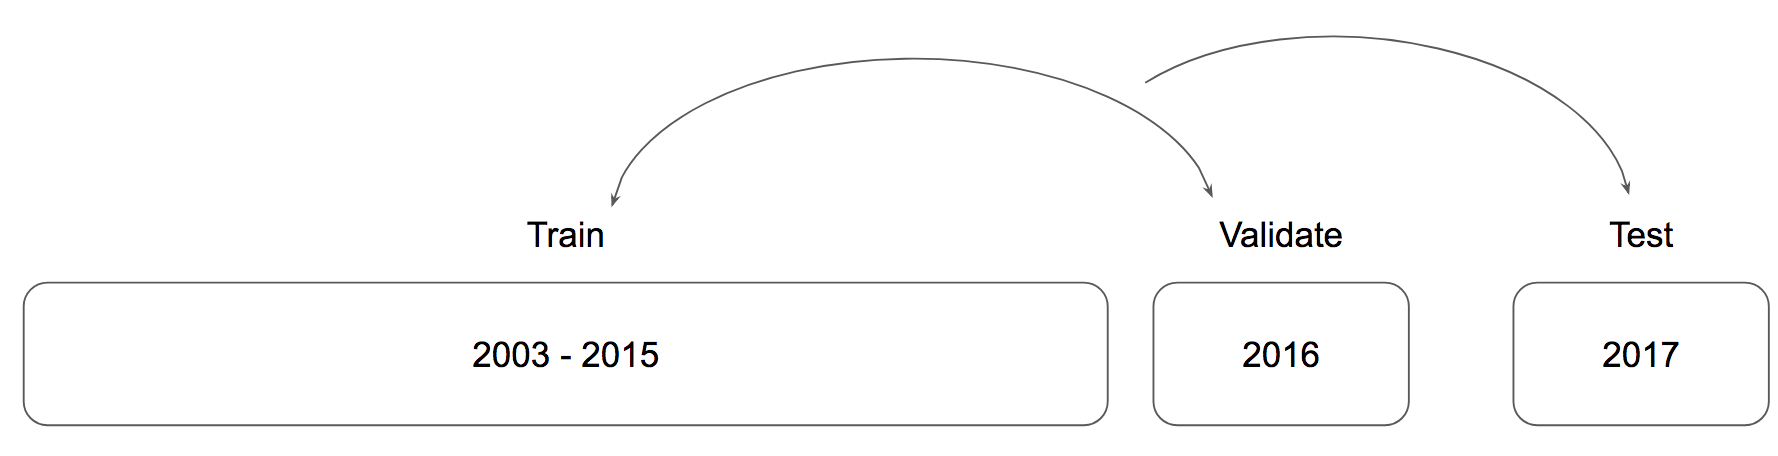
\includegraphics[width=1\linewidth]{Sections/tables and figures/Train Validate Test} \caption{Out-of-time validation}\label{fig:TrainTestValidate}
\end{figure}

\section{Results}\label{results}

\subsection{Probability of Sale Model}\label{probability-of-sale-model}

\subsection{Sale Price Model}\label{sale-price-model}

\subsection{Using the Models in
Practice}\label{using-the-models-in-practice}

\section{Conclusions and Future
Research}\label{conclusions-and-future-research}

\subsection{Future Research}\label{future-research}

\subsection{Conclusion}\label{conclusion}

\section*{References}\label{references}
\addcontentsline{toc}{section}{References}

\hypertarget{refs}{}
\hypertarget{ref-Almanie2015}{}
Almanie, R.; Lor, T.; Mirza. 2015. ``Crime Prediction Based on Crime
Types and Using Spatial and Temporal Criminal Hotspots.''
\emph{International Journal of Data Mining \& Knowledge Management
Process (IJDKP)} 5 (4).

\hypertarget{ref-antipov12}{}
Antipov, Evgeny A., and Elena B. Pokryshevskaya. 2012. ``Mass Appraisal
of Residential Apartments: An Application of Random Forest for Valuation
and a Cart-Based Approach for Model Diagnostics.'' \emph{Expert Systems
with Applications}.

\hypertarget{ref-Pollack2010}{}
Barry Bluestone \& Chase Billingham, Stephanie Pollack \&. 2010.
``Maintaining Diversity in America's Transit-Rich Neighborhoods: Tools
for Equitable Neighborhood Change.'' \emph{New England Community
Developments, Federal Reserve Bank of Boston}, 1--6.

\hypertarget{ref-Breiman2001}{}
Breiman, L. 2001. ``Random Forests.'' \emph{Machine Learning} 45 (1):
5--32.

\hypertarget{ref-Chapple2009}{}
Chapple, Karen. 2009. ``Mapping Susceptibility to Gentrification: The
Early Warning Toolkit.'' \emph{Berkeley, CA: Center for Community
Innovation.}

\hypertarget{ref-Chapple2016}{}
Chapple, Miriam, Karen; Zuk. 2016. ``Forewarned: The Use of Neighborhood
Early Warning Systems for Gentrification and Displacement.''
\emph{Cityscape: A Journal of Policy Development and Research} 18 (3).

\hypertarget{ref-Clay1979}{}
Clay, Phillip L. 1979. \emph{Neighborhood Renewal: Middle-Class
Resettlement and Incumbent Upgrading in American Neighborhoods}.
Lexington Books.

\hypertarget{ref-Dietzell2014}{}
Dietzell, Nicole; Schäfers, Marian Alexander; Braun. 2014.
``Sentiment-Based Commercial Real Estate Forecasting with Google Search
Volume Data.'' \emph{Journal of Property Investment \& Finance,} 32 (6):
540--69.

\hypertarget{ref-Dreier2004}{}
Dreier, John; Swanstrom, Peter; Mollenkopf. 2004. \emph{Place Matters:
Metropolitics for the Twenty-First Century.} University Press of Kansas.

\hypertarget{ref-Springer2017}{}
d'Amato, Tom, Maurizio; Kauko, ed. 2017. \emph{Advances in Automated
Valuation Modeling}. Springer International Publishing.

\hypertarget{ref-Eckert1990}{}
Eckert, J. K. 1990. \emph{Property Appraisal and Assessment
Administration}. Chicago, IL.: International Association of Assessing
Officers.

\hypertarget{ref-Fotheringham2015}{}
Fotheringham, R; Yao, A.S.; Crespo. 2015. ``Exploring, Modelling and
Predicting Spatiotemporal Variations in House Prices.'' \emph{The Annals
of Regional Science} 54.

\hypertarget{ref-Fu2014}{}
Fu, Yanjie; et al. 2014. \emph{Exploiting Geographic Dependencies for
Real Estate Appraisal: A Mutual Perspective of Ranking and Clustering}.
Proceedings of the 20th ACM SIGKDD international conference on Knowledge
discovery; data mining.

\hypertarget{ref-Geltner2017}{}
Geltner, David, and Alex Van de Minne. 2017. ``Do Different Price Points
Exhibit Different Investment Risk and Return Commercial Real Estate.''
Real Estate Research Institute.

\hypertarget{ref-Guan2014}{}
Guan, Jian, Donghui Shi, Jozef M. Zurada, and Alan S. Levitan. 2014.
``Analyzing Massive Data Sets: An Adaptive Fuzzy Neural Approach for
Prediction, with a Real Estate Illustration.'' \emph{Journal of
Organizational Computing and Electronic Commerce} 24 (1). Taylor \&
Francis: 94--112.
doi:\href{https://doi.org/10.1080/10919392.2014.866505}{10.1080/10919392.2014.866505}.

\hypertarget{ref-Helbich2013}{}
Helbich, et al., Marco. 2013. ``Boosting the Predictive Accuracy of
Urban Hedonic House Price Models Through Airborne Laser Scanning.''
\emph{Computers, Environment and Urban Systems} 39: 81--92.

\hypertarget{ref-Johnson2007}{}
Johnson, Ken, Justin Benefield, and Jonathan Wiley. 2007. ``The
Probability of Sale for Residential Real Estate.'' \emph{Journal of
Housing Research} 16 (2): 131--42.
doi:\href{https://doi.org/10.5555/jhor.16.2.0234g75800h5k8x6}{10.5555/jhor.16.2.0234g75800h5k8x6}.

\hypertarget{ref-Kontrimasa2011}{}
Kontrimasa, Antanas, Vilius; Verikasb. 2011. ``The Mass Appraisal of the
Real Estate by Computational Intelligence.'' \emph{Applied Soft
Computing}.

\hypertarget{ref-Koschinsky2012}{}
Koschinsky, J. et al. 2012. ``The Welfare Benefit of a Home's Location:
An Empirical Comparison of Spatial and Non-Spatial Model Estimates.''
\emph{Journal of Geographical Systems} 10109.

\hypertarget{ref-Lees2008}{}
Lees, Tom; Wyly, Loretta; Slater. 2008. ``Gentrification.'' \emph{Growth
and Change} 39 (3): 536--39.
doi:\href{https://doi.org/10.1111/j.1468-2257.2008.00443.x}{10.1111/j.1468-2257.2008.00443.x}.

\hypertarget{ref-Miller2015}{}
Miller, J.; Aspinall, J.; Franklin. 2007. ``Incorporating Spatial
Dependence in Predictive Vegetation Models.'' \emph{Ecological
Modelling} 202 (3): 225--42.

\hypertarget{ref-Park2015}{}
Park, Jae Kwon, Byeonghwa; Bae. 2015. ``Using Machine Learning
Algorithms for Housing Price Prediction: The Case of Fairfax County,
Virginia Housing Data.'' \emph{Expert Systems with Applications} 42 (6):
2928--34.

\hypertarget{ref-Pivo2011}{}
Pivo, Gary, and Jeffrey D. Fisher. 2011. ``The Walkability Premium in
Commercial Real Estate Investments.'' \emph{Real Estate Economics} 39
(2): 185--219.
doi:\href{https://doi.org/10.1111/j.1540-6229.2010.00296.x}{10.1111/j.1540-6229.2010.00296.x}.

\hypertarget{ref-Rafiei2016}{}
Rafiei, Hojjat, Mohammad Hossein; Adeli. 2016. ``A Novel Machine
Learning Model for Estimation of Sale Prices of Real Estate Units.''
\emph{Journal of Construction Engineering and Management} 142 (2).

\hypertarget{ref-Reardon2011}{}
Reardon, Kendra, Sean F.; Bischoff. 2011. ``Income Inequality and Income
Segregation.'' \emph{American Journal of Sociology}.

\hypertarget{ref-Schernthanner2016}{}
Schernthanner H., Gonschorek J., Asche H. 2016. ``Spatial Modeling and
Geovisualization of Rental Prices for Real Estate Portals.''
\emph{Computational Science and Its Applications} 9788.

\hypertarget{ref-Silverherz1936}{}
Silverherz, J. D. 1936. ``The Assessment of Real Property in the United
States.'' \emph{Albany: J.B. Lyon Co. Printers}.

\hypertarget{ref-Smith1979}{}
Smith, Neil. 1979. ``Toward a Theory of Gentrification a Back to the
City Movement by Capital, Not People.'' \emph{Journal of the American
Planning Association} 45 (4). Routledge: 538--48.
doi:\href{https://doi.org/10.1080/01944367908977002}{10.1080/01944367908977002}.

\hypertarget{ref-urban2016}{}
Solomon Greene, Molly Scott, Rolf Pendall, and Serena Lei. 2016. ``Open
Cities: From Economic Exclusion to Urban Inclusion.'' \emph{Urban
Institue Brief}, June. Urban Institue Brief.

\hypertarget{ref-Turner2001}{}
Turner, Margery Austin, and Christopher Snow. 2001. \emph{Leading
Indicators of Gentrification in d.C. Neighborhoods}.

\hypertarget{ref-Watson2009}{}
Watson, Tara. 2009. ``Inequality and the Measurement of Residential
Segregation by Income in American Neighborhoods.'' \emph{Review of
Income and Wealth}.

\hypertarget{ref-Zuk2015}{}
Zuk, Miriam; et al. 2015. ``Gentrification, Displacement and the Role of
Public Investment: A Literature Review.''


\end{document}
